\documentclass[../main.tex]{subfiles}
\begin{document}
\chapter{The Large Hadron Collider and the CMS experiment}
\label{intro:chap:exp}

\section{The Large Hadron Collider}
\label{intro:sec:lhc}

The Large Hadron Collider (LHC) is the most powerful particle accelerator ever built \cite{intro:exp:lhc}. It's located at CERN (\textit{Organisation européenne pour la recherche nucléaire}, European Organization for Nuclear Research) in the border between France and Switzerland, near Geneva. The accelerator is a 27~km circular collider built around 100~m underground composed by two rings where two beams of protons or heavy ions circulate in opposite directions inside vacuum pipes. The beams are bended using 1232 superconducting dipoles, cooled down with superfluid helium to 1.9~K, which generate an 8.3~T magnetic field. To focus the beams and avoid spreading, 392 quadrupole magnets are used.

The LHC is the last step of the accelerating chain in which the particles reach the operating energies. The CERN accelerator complex is shown in Fig.~\ref{intro:exp:cern_acc_chain}. At the beginning of the chain, hydrogen atoms are ionized and injected into the LINAC2, where they are accelerated to an energy of around 50~MeV. Then, the beam is passed through a series of circular synchrotrons, reaching 1.4~GeV after the BOOSTER, 26~GeV after the PS and 450~GeV after the SPS, before they enter into the LHC and reach their target energy. The designed center-of-mass energy ($\sqrt{s}$) for proton-proton collisions is 14 TeV, although the target energy has changed over the different phases: 7~TeV during 2010 and 8~TeV during 2011 and 2012 (3-year period called Run 1), 13~TeV during Run 2 (2015-2018) and 13.6~TeV during Run 3 (which started in 2022).

\begin{figure}[h!]
\begin{center}
\includegraphics[width=0.7\textwidth]{Images/CCC-v2018-print-v2}
\end{center}
\caption[CERN accelerator complex]{CERN accelerator complex. Extracted from \cite{intro:exp:cern_acc_chain_image}.}
\label{intro:exp:cern_acc_chain}
\end{figure}

The beams are made to intersect at four points in the LHC, where the four experiments are placed. ATLAS (\textit{A Toroidal LHC ApparatuS}) and CMS (\textit{Compact Muon Solenoid}) are two general purpose experiments with similar physics programs located in opposite sites of the LHC ring. ALICE (\textit{A Large Ion Collider Experiment}) is focused mostly on heavy ion collision in order to study quark-gluon plasma, while LHCb (\textit{LHC beauty}) focuses on CP-violation and the matter-antimatter asymmetry by studying \textit{b} quark physics.

\subsection{Luminosity}

In the beams, \textit{bunches} are formed by grouping $n$ protons within a 25~ns time spacing ($\Delta t_0$), so the probability of interaction between the beams when they collide increases. Sets of consecutive bunches are further structured in \textit{trains}. A \textit{fill} is defined as the period of data taking between the beam is injected in the accelerator until it is dumped. 

The beam's main properties are the transverse emittance, $\epsilon$, which reflects how close two protons in the same bunch are in the position-momentum phase space; and the amplitude function, $\beta^*$, which defines how focused the beam is.


The instantaneous luminosity, $L_{ins}$, determines the amount of collisions produced per unit of time and area. It can be obtained considering the previously described design and operation parameters and is given by,
\begin{equation}
L_{ins} = \frac{n_1 n_2 f}{4\Delta\epsilon\beta^*},
\label{intro:eq:lumi_inst}
\end{equation}
where $n_1$ and $n_2$ are the number of protons in the two bunches that collide and $f$ is the beam frequency. Typical values for these parameters during Run 2 are $n=1.2\times10^{11}$ protons per bunch, $f=40~$MHz, $\epsilon=3.75$~mm$\times\mu$rad and $\beta^*=0.55$~m, which give a nominal instantaneous luminosity in the order of $10^{34}$~cm${}^{-2}$s${}^{-1}$, with a maximum obtained during Run 2 of $\sim2\times10^{34}$~cm${}^{-2}$s${}^{-1}$. 

For a given process with cross section $\sigma$, the expected number of events is given by
\begin{equation}
\frac{dN}{dt} = \sigma L_{ins},
\end{equation}
so, in order to study physical processes with low production cross section, a high luminosity is needed. The total number of $pp$ events is proportional to the integrated luminosity:
\begin{equation}
L_{int} = \int L_{ins}~dt.
\end{equation}

Fig.~\ref{intro:fig:lumi_int} shows the total integrated luminosity delivered by the LHC and the recorded by the CMS experiment during the Run 2 data taking period.

\begin{figure}[h!]
\begin{center}
\includegraphics[width=0.7\textwidth]{Images/int_lumi_allcumulative_pp_run2}
\end{center}
\caption[Integrated luminosity during Run 2]{Integrated luminosity delivered by the LHC and recorded by the CMS experiment during the Run 2 data taking period. Extracted from \cite{intro:exp:cms_lumi}.}
\label{intro:fig:lumi_int}
\end{figure}



The average number of simultaneous interactions per bunch crossing, i.e. the pile-up (PU), is obtained as
\begin{equation}
\langle PU \rangle = \frac{L_{ins}~\sigma_{pp}^{inel}~\Delta t_0}{n},
\end{equation}
where $\sigma_{pp}^{inel}$ is the inelastic $pp$ cross section. High PU values result in a very high detector occupancy, which degrades the efficiency and resolution of the particle reconstruction. Fig.~\ref{intro:fig:pu} shows the PU distributions during the Run 2 data-taking period. 

\begin{figure}[h!]
\begin{center}
\includegraphics[width=0.7\textwidth]{Images/pu}
\end{center}
\caption[Run 2 pile-up distribution]{Distribution of the average number of interactions per crossing (pile-up) for pp collisions in 2015 (purple), 2016 (orange), 2017 (light blue), 2018 (navy blue), and the full Run 2 period (gray).}
\label{intro:fig:pu}
\end{figure}



\subsection{The High Luminosity LHC}
\label{intro:sec:hllhc}

Throughout the lifetime of the LHC, several improvements on the accelerator have been implemented during long shutdowns (LS) in order to extend its discovery potential, as displayed on the roadmap in Fig.~\ref{intro:exp:lhc_roadmap}. In LS1, the interconnections between the LHC superconducting magnets were consolidated to increase the center-of-mass energy to 13 TeV and allowing the machine to reach instantaneous luminosities of up to $2.1\times10^{34}$~cm${}^{-2}$s${}^{-1}$, equivalent to an average pile-up of 55. During LS2, an optimization of the LHC parameters was performed so the machine can increase its center-of-mass energy to 13.6~TeV and sustain a maximum instantaneous luminosity of $2\times10^{34}$~cm${}^{-2}$s${}^{-1}$ during longer periods of time during Run-3. The next long shutdown, LS3, will include a major upgrade to both the accelerator and the experiments, starting the Phase 2 operation of the LHC or High Luminosity LHC (HL-LHC) \cite{intro:exp:hllhc}. In its nominal operation, the accelerator will run at a centre-of-mass energy of up to 14 TeV, while the instantaneous luminosity will increase during Run 4 up to $5-7.5\times10^{34}$~cm${}^{-2}$s${}^{-1}$, corresponding to a PU of 140-200, potentially leading to a total integrated luminosity of up to 4000~fb${}^{-1}$ after 10 years of operations. This increase needs to be addressed by corresponding detector upgrades in order to be able to cope with the higher instantaneous and integrated luminosities and maintain the performance of the reconstruction system in this new PU scenario.

\begin{figure}[h!]
\begin{center}
\includegraphics[width=\textwidth]{Images/HL-LHC_Janvier2022}
\end{center}
\caption[LHC baseline schedule]{LHC baseline plan for the next decade and beyond showing the collision energy (upper line), the instantaneous luminosity (lower line) and the total integrated luminosity (lower boxes). Running periods and long shutdowns are also displayed.}
\label{intro:exp:lhc_roadmap}
\end{figure}



\section{The CMS experiment}

The CMS detector \cite{intro:exp:cms} is a general-purpose experiment located 100~m underground at the LHC point 5, near the french village of Cessy. The apparatus is a cylindrical detector with a length of 21.6~m and a diameter of 14.6~m. Its main feature is the presence of a superconducting solenoid of 6 m internal diameter and 12.5~m length, which creates an homogeneous magnetic field of 3.8~T. The intense magnetic field allows to measure the transverse momentum and the electric charge of charged particles from their curved trajectories.

\subsection{Coordinate system}

The CMS experiment uses a right-handed coordinate system centred in the nominal interaction point. The $x$-axis points towards the centre of the LHC ring, the $y$-axis vertically and the $z$-axis along the beam direction. Polar coordinates are usually used, so the azimuthal angle $\phi$ is defined in the $xy$ plane by the angle with respect to the $x$-axis and the polar angle $\theta$ is defined in the $rz$ plane as the angle formed with the $z$-axis. An schematic of this coordinate system is shown in Fig.~\ref{intro:exp:cms_coords}.

\begin{figure}[h!]
\begin{center}
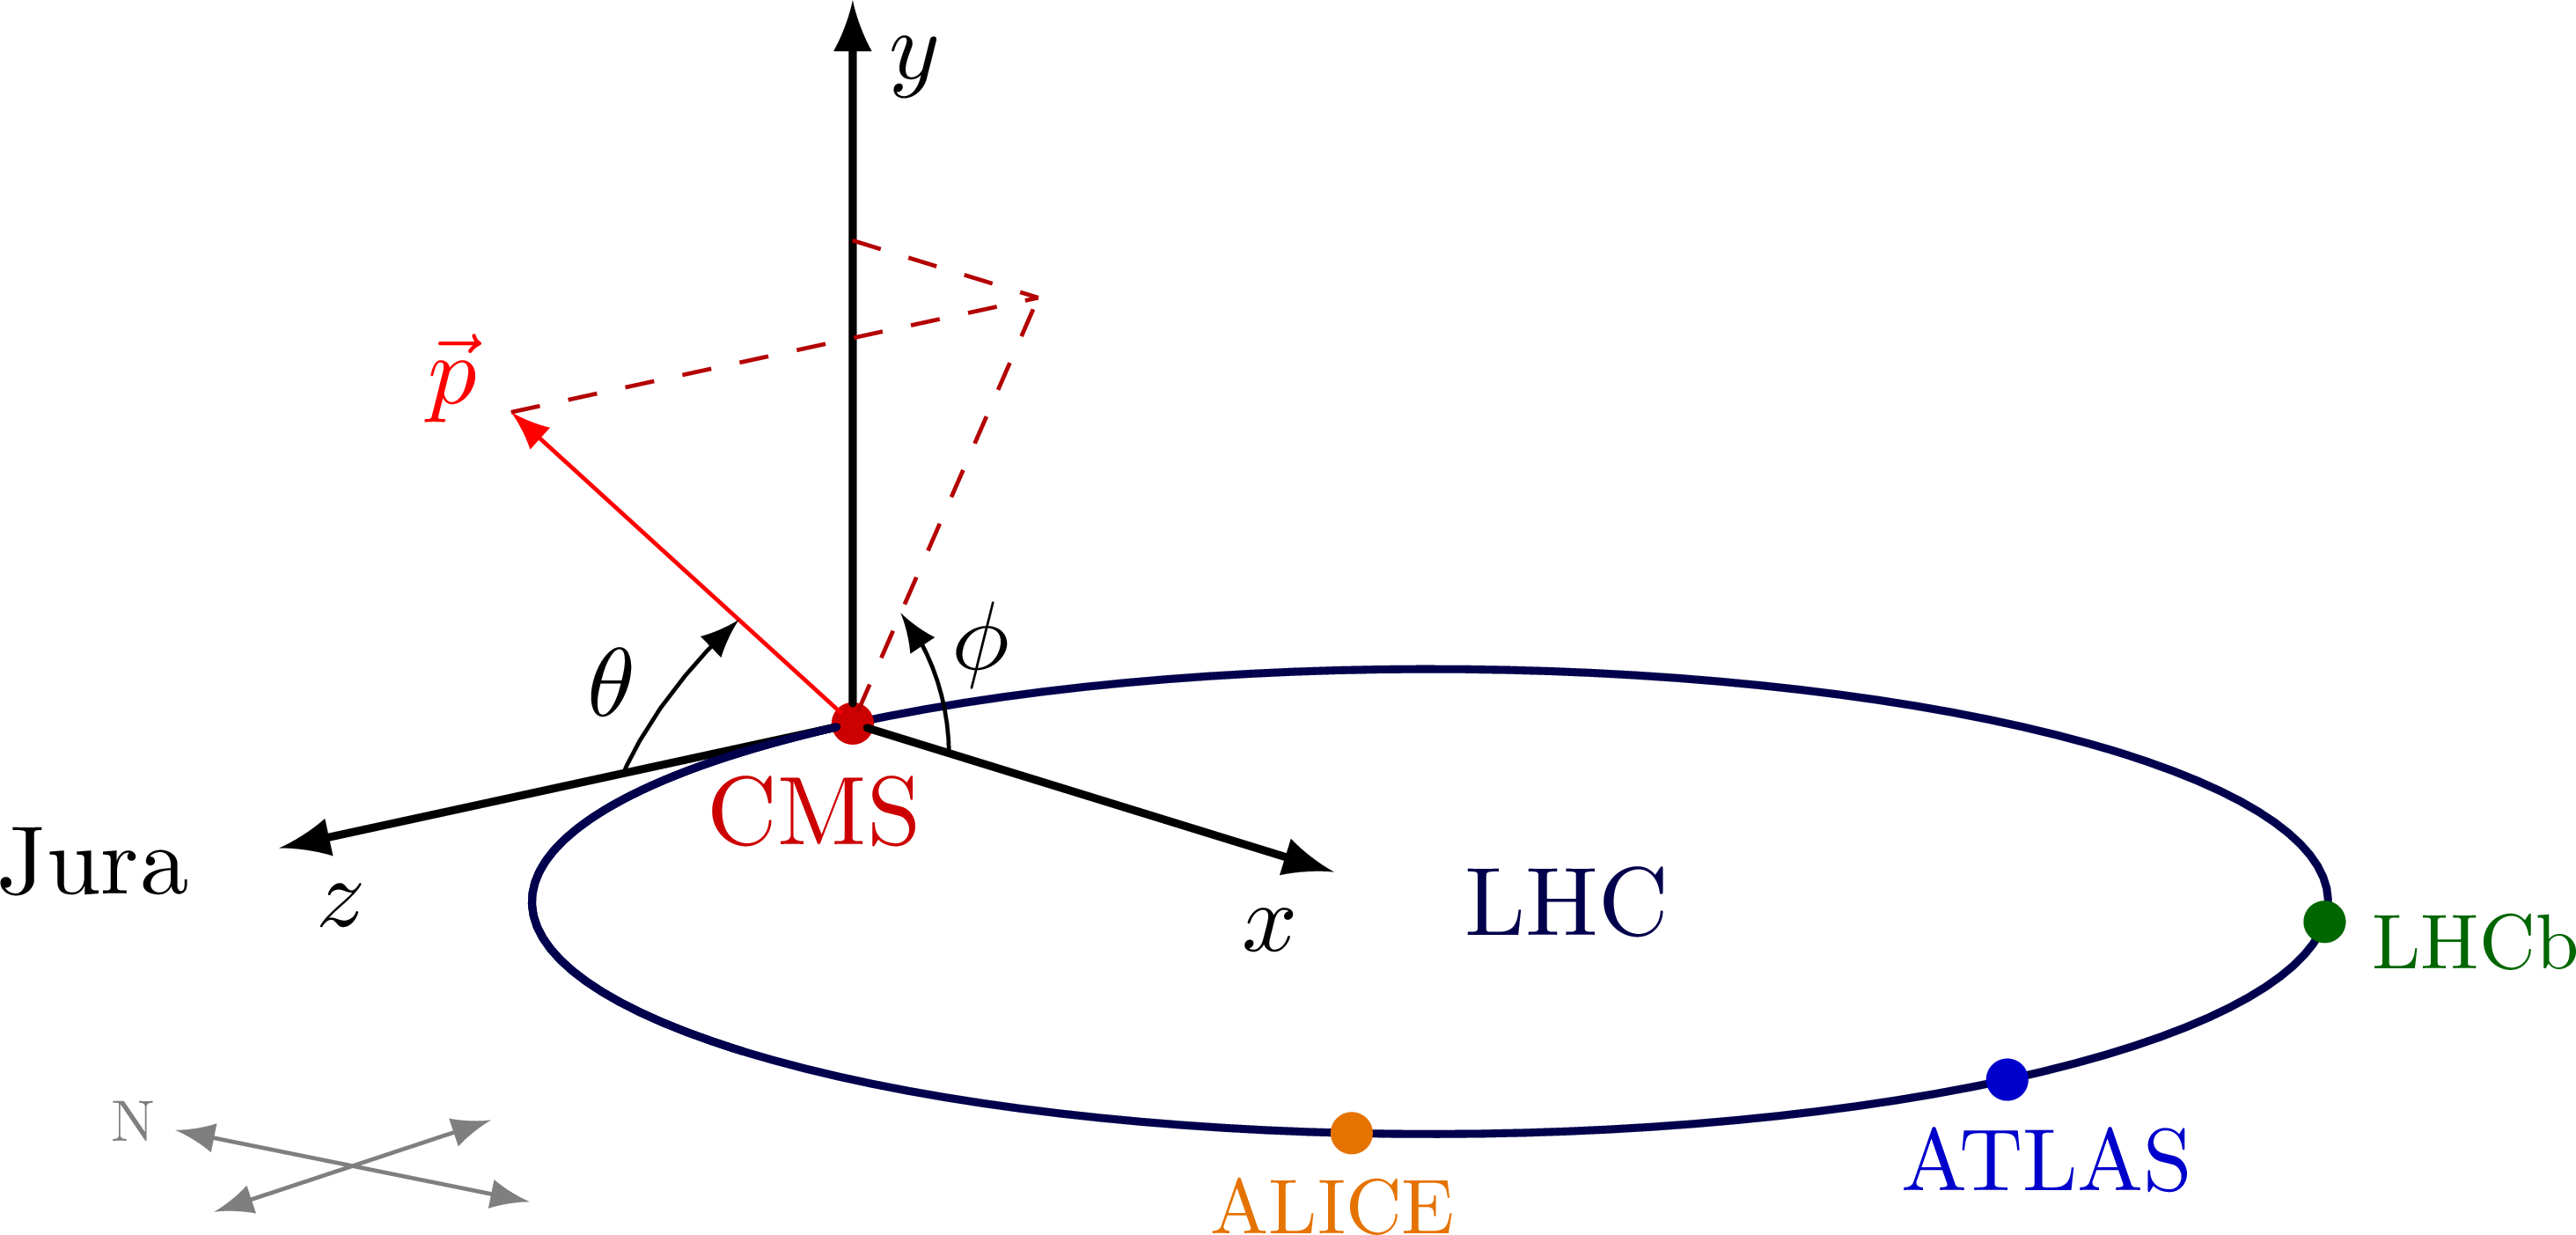
\includegraphics[width=0.5\textwidth]{Images/axis3D_CMS-002}
\end{center}
\caption[CMS coordinate system]{Illustration of the CMS coordinate system. Extracted from \cite{intro:exp:cms_coord}.}
\label{intro:exp:cms_coords}
\end{figure}

The \textit{rapidity} $y$ is defined as
\begin{equation}
y = \frac{1}{2}\ln\left(\frac{E+p_z}{E-p_z}\right),
\end{equation}
where $E$ and $p_z$ are the energy and the momentum along the beam axis respectively for a given particle. Differences in rapidity are invariant under Lorentz boosts, so this variable is very useful in hadronic collision studies. Instead of this variable, for highly relativistic particles an approximated quantity called the \textit{pseudorapidity} $\eta$ can be used:
\begin{equation}
\eta = -\ln\left(\tan \frac{\theta}{2} \right),
\end{equation}
which does not depend on the particle energy or momentum. Pseudorapidity varies from 0 when $\theta=\pi/2$ to infinity when $\theta=0$. Regions with large $|\eta|$ are often referred to as \textit{forward}, while the ones with low $|\eta|$, as \textit{central}.

Using the angle $\phi$, the pseudorapidity $\eta$ and the momentum in the plane orthogonal to the beam axis $p_T$ (\textit{transverse momentum}), the particle's momentum can be completely defined. They are related to the usual $p_x$, $p_y$ and $p_z$ by
\begin{align}
p_x = p\sin\theta\cos\phi = p_T \cos\phi, \\
p_y = p\sin\theta\sin\phi = p_T \sin\phi, \\
p_z = p\cos\phi = p_T \sinh \eta.
\end{align}

Another variable that will be useful later is the angular distance $\Delta R$ between two particles with coordinates $(\eta_1, \phi_1)$ and $(\eta_2, \phi_2)$,
\begin{equation}
\Delta R = \sqrt{(\eta_1 - \eta_2)^2 + (\phi_1 - \phi_2)^2}.
\end{equation}
This variable is usually considered to perform jet clustering or to evaluate the \textit{isolation} of a particle with respect to its neighbouring particles, i.e. the amount of energy found in a cone around the particle.  This metric helps to discriminate between \textit{prompt} particles (i.e. coming from the hard interaction) from particles found inside jets or coming from soft scattering.


\subsection{Subdetectors}

The structure of the CMS detector is shown in Fig.~\ref{intro:fig:subdetectors}. The central zone of the detector, or \textit{barrel}, is divided intro cylindrical slices, called \textit{wheels}. Each wheel is numbered from -2 to 2, being wheel 0 the one where the interaction point is located. The two forward regions, beyond wheels -2 and 2, are called the \textit{endcaps}.


\begin{figure}[h!]
\begin{center}
\includegraphics[width=\textwidth]{Images/cms_160312_02}
\end{center}
\caption[CMS subdetectors]{Schematic layout of the CMS subdetectors. Extracted from \cite{intro:exp:subdetectors}.}
\label{intro:fig:subdetectors}
\end{figure}

The detector is composed by several subdetectors nested around the interaction point, each with a different technology to detect different kinds of particles. Ordered by vicinity to the interaction point, they are located both before (silicon tracker, electromagnetic calorimeter and hadronic calorimeters) and after (muon system) the magnetic solenoid. A description of each subdetector (starting from the solenoid magnet) is included in the following.

\subsubsection{The solenoid magnet}

The solenoid magnet is the central feature of the CMS detector. It is a niobium-titanium superconducting solenoid operating at 4.5~K. It provides a 3.8~T magnetic field inside the solenoid and up to 2~T outside it. The return yoke of the magnet is made of steel, and is located between the chambers of the muon system.

The magnetic field bends the trajectory of charged particles produced in the collision, and their transverse momentum can be inferred from the curvature of their trajectory. A larger magnetic field produces a larger bending, increasing the precision on the momentum determination. 

\subsubsection{The silicon tracker}

The CMS tracker \cite{intro:exp:tracker1, intro:exp:tracker2} is the innermost part of the CMS detector. It has a diameter of 2.5~m and a length of 5.8~m, covering up to $|\eta|<2.5$. It's built in silicon, so it can resist well the high radiation levels produced during the collisions while providing very good spatial resolution. When charged particles transverse the tracker volume, they deposit their energy by ionizing the silicon semiconductors, creating electron-hole pairs that induce currents that drift to the electrodes, where they are digitized and measured. These \textit{hits} can be combined into \textit{tracks} by using pattern recognition algorithms (see Section~\ref{intro:sec:id}) to reconstruct both its trajectory and origin. This origin could be the main interaction point, or \textit{primary vertex}, or \textit{secondary vertices} displaced a few millimetres from the primary vertex. These secondary vertices are produced from the decay of particles like heavy-flavour quarks or $\tau$ leptons.

A structural view of the tracker is shown in Fig.~\ref{intro:fig:tracker}. It consists of two main detectors: a pixel detector surrounding the beam pipe and a strip detector surrounding the pixel detector.

\begin{figure}[h!]
\begin{center}
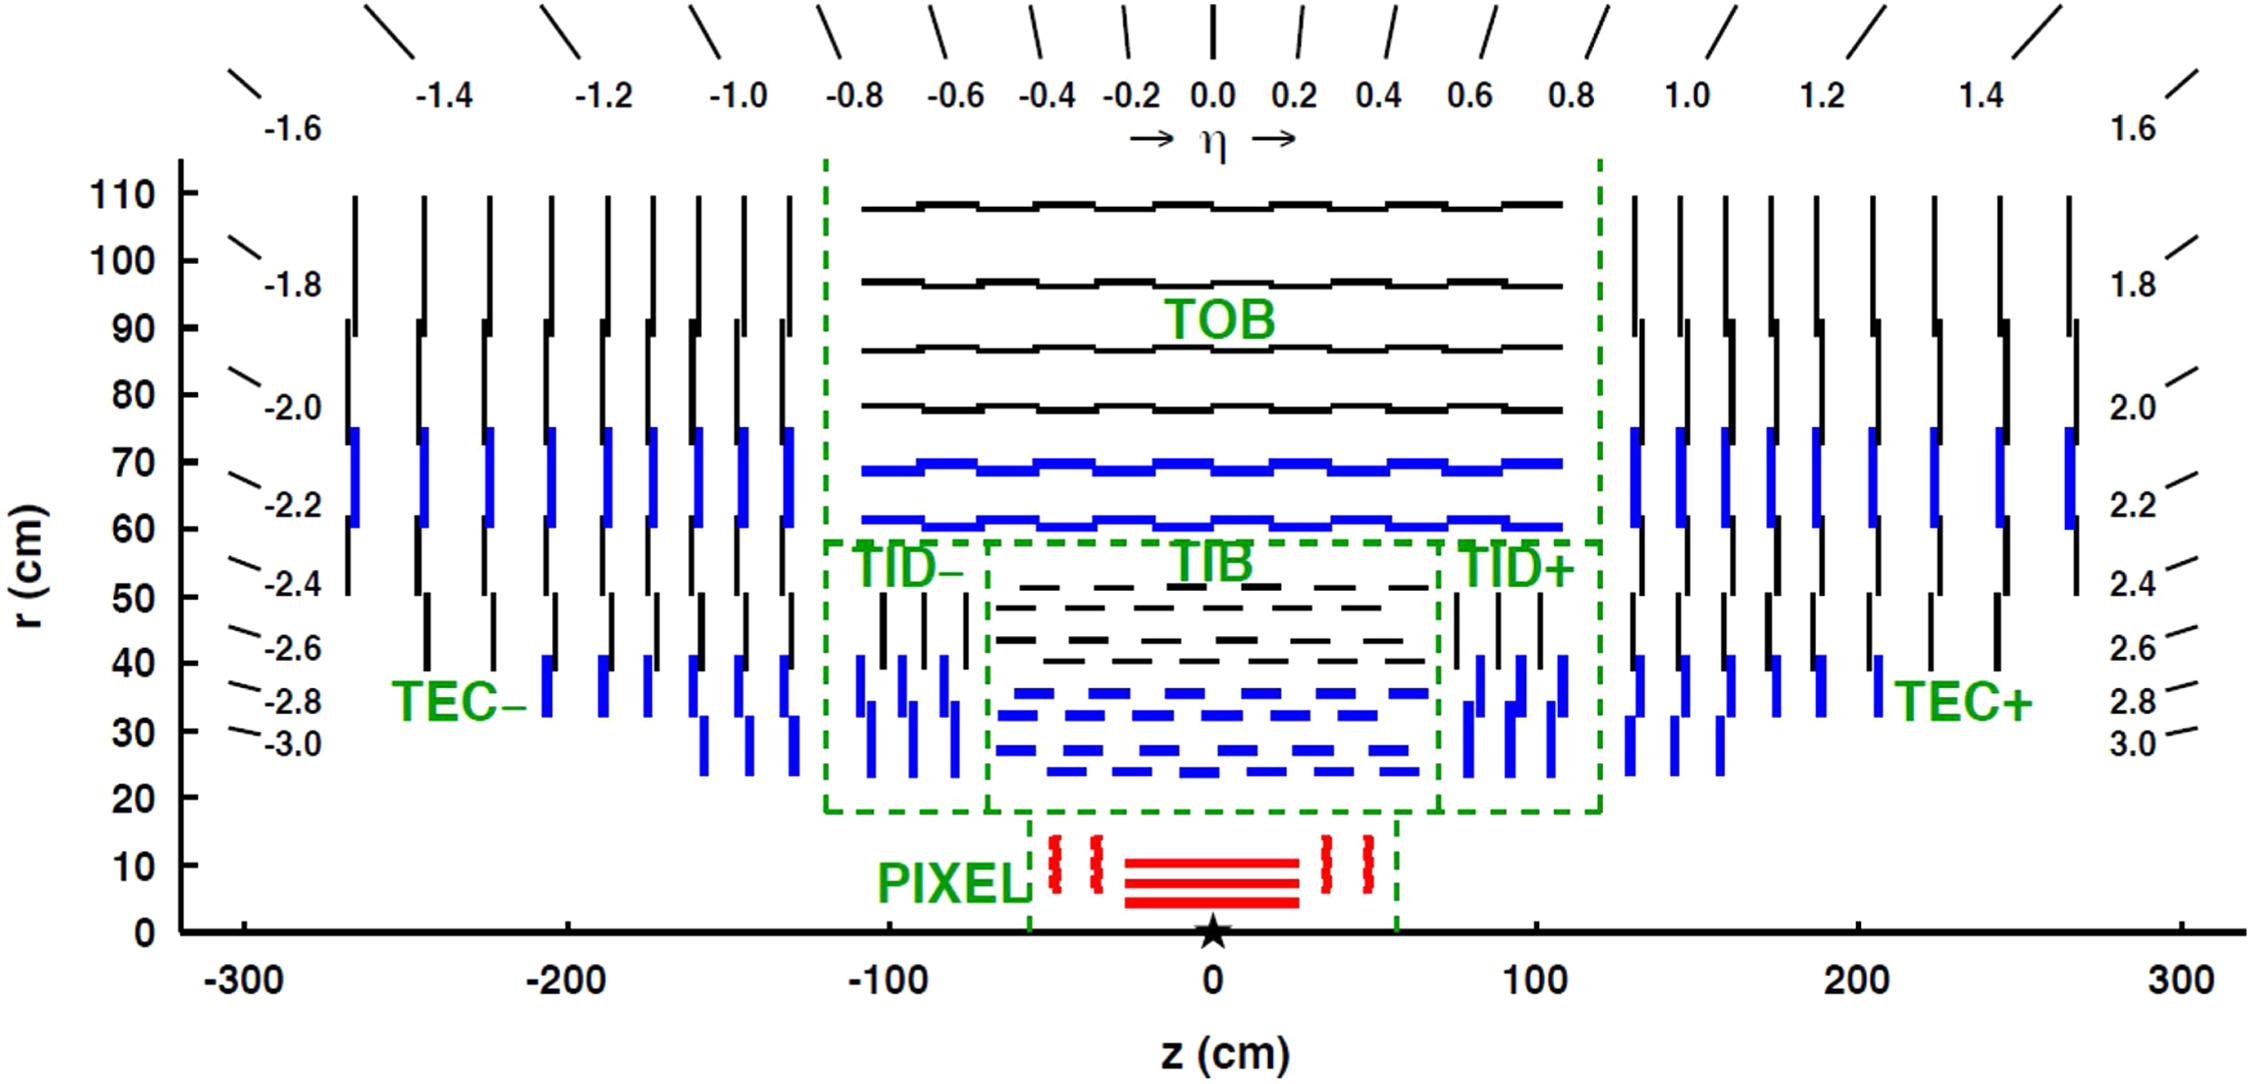
\includegraphics[width=\textwidth]{Images/tracker}
\end{center}
\caption[CMS tracker structure]{Schematic structure of a tracker slice in the $r$-$z$ plane. Extracted from \cite{intro:exp:tracker3}}
\label{intro:fig:tracker}
\end{figure}

The pixel tracker covers the innermost region of the tracker, where the flux of particles coming from the collisions is higher. At these small distances to the interaction point, a very high granularity is then needed in order to resolve hits of neighbouring particles. The detector originally consisted of three detector layers in the barrel region with radii 4.4, 7.3, and 10.2~cm, and two layers on each side of the detector at distances of $\pm34.5$~cm and $\pm46.5$~cm. An upgrade on the detector was performed before the 2017 data-taking period \cite{intro:exp:tracker_upgrade}, so a high tracking performance could be maintained when reaching luminosities up to $2\times10^{34}$~cm${}^{-2}$s${}^{-1}$ and $|\text{PU}|$ exceeding 50. In this upgrade, the detector was replaced with four barrel and three endcap layers on each side. A comparison between before and after the upgrade is shown in Fig.~\ref{intro:fig:tracker_upgrade}. A total of 124 million pixels are included in the upgraded pixel detector, each with a 100$\times$150~$\mu$m${}^2$ cross section. The detector produces 3-D measurements along the paths of the charged particles with single hit resolutions around 10~$\mu$m.

\begin{figure}[h!]
\begin{center}
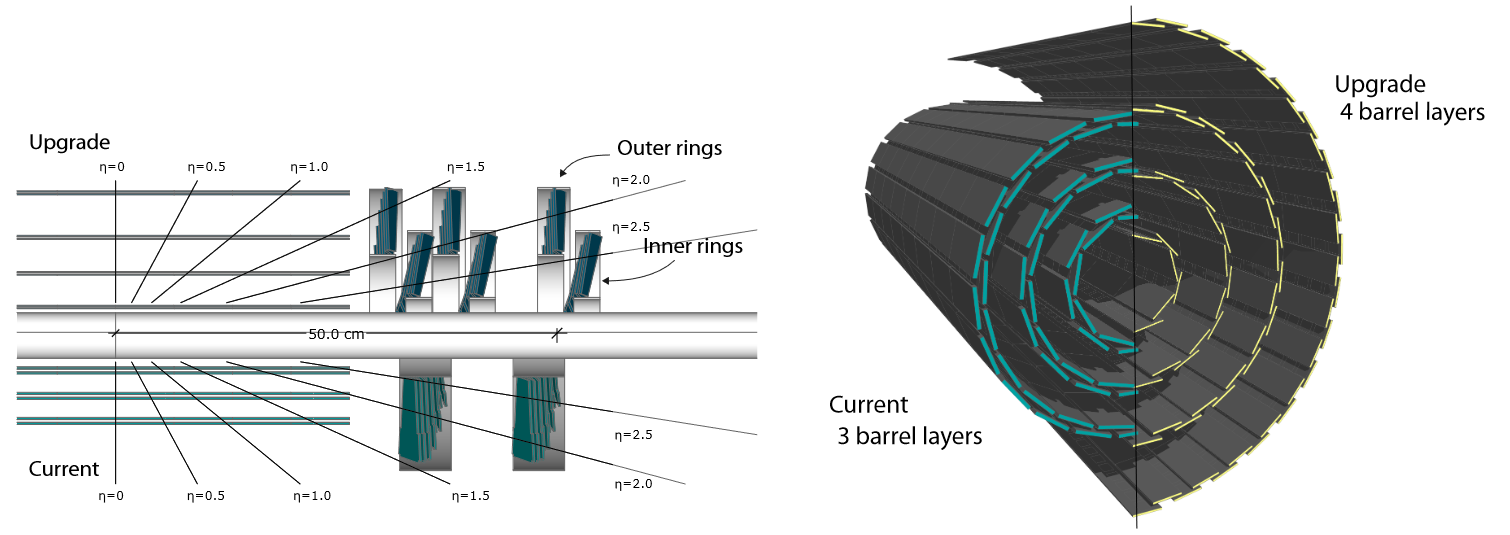
\includegraphics[width=\textwidth]{Images/tracker_upgrade}
\end{center}
\caption[CMS pixel detector upgrade]{Comparison of the pixel detector before and after to 2017 upgrade (labeled as \textit{Current} and \textit{Upgrade} respectively). Extracted from \cite{intro:exp:tracker_upgrade}.}
\label{intro:fig:tracker_upgrade}
\end{figure}

In the outer part of the tracking system, the strip detector consists of 9.3 million silicon micro-strip sensors. Given the lower occupancy in this region, the use of microstrips is enough to provide an unambiguous hit detection. The strip tracker is divided into four regions with different layouts. In the barrel, the Tracker Inner Barrel (TIB) covers the region of radii between 20 and 55~cm, while the Tracker Outer Barrel (TOB) reaches up to $r=116$~cm. They contain four and six layers respectively. In the endcaps, the TIB is covered by the Tracker Inner Disk (TID), made out of three layers on each side of the detector, ant the Tracker Endcaps (TEC) in the forward regions, with nine layers. The TIB and TID provide single hit position resolutions of around 13-38~$\mu$m, while the TEC and TOB, approximately 18-47~$\mu$m.


\subsubsection{The Electromagnetic Calorimeter}

The Electromagnetic Calorimeter (ECAL) \cite{intro:exp:ecal} is a hermetic and homogeneous array of lead tungstate (PbWO${}_4$) scintillating crystals. It is designed so an incident electron or photon generates an electromagnetic shower that deposits most of its energy inside the ECAL volume.  With the location and magnitude of the energy deposits, the energy and the direction of the incident particle can be measured. The characteristics of the PbWO${}_4$ crystals make them an appropriate choice for kind of operation at the LHC, thanks to its high density (8.28~g/cm${}^{3}$), short radiation length (0.89~cm) and small Molière radius (2.2~cm), resulting in a fine granularity and a compact calorimeter.

The ECAL layout is shown in Fig.~\ref{intro:fig:ecal}. It is divided in three different regions: the barrel ECAL (EB) ($|\eta|<1.4.79$), two endcaps (EE), with a  $1.57 < |\eta|<3$ coverage, and a preshower detector (ES) in front of the endcaps ($1.65 < |\eta| < 2.6$).


\begin{figure}[h!]
\begin{center}
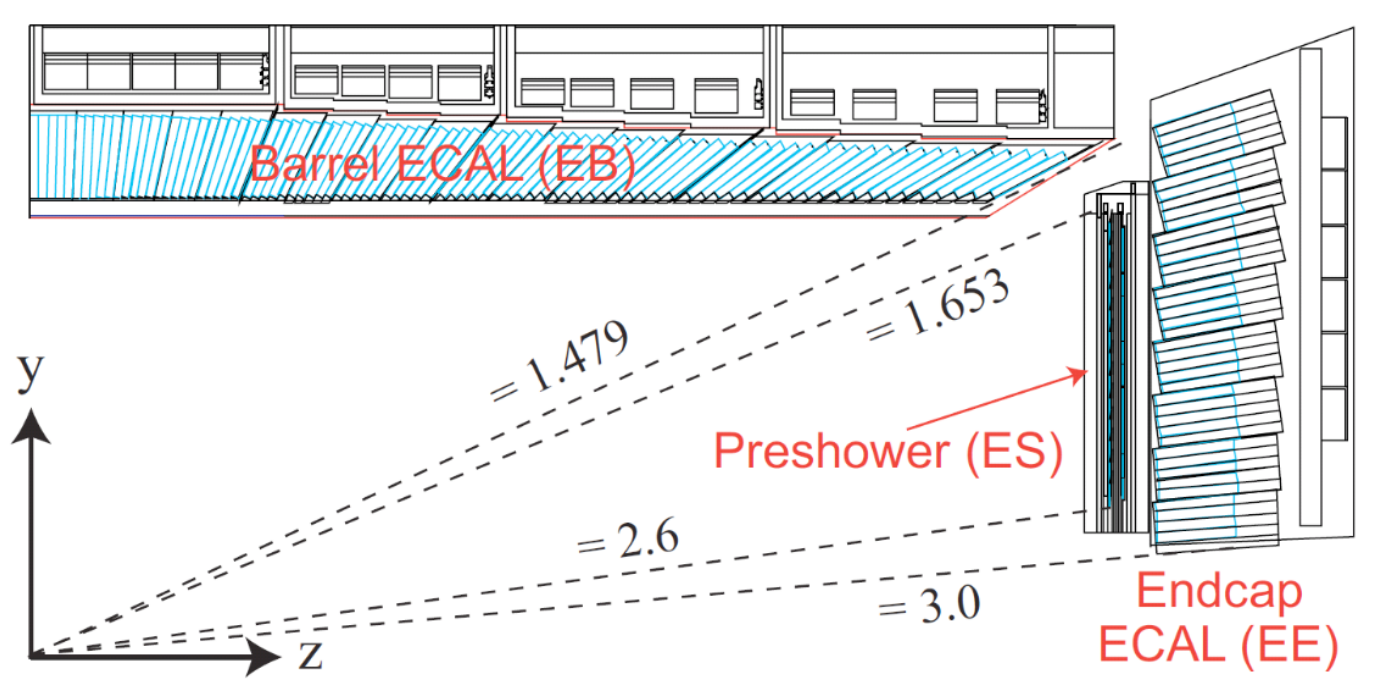
\includegraphics[width=0.6\textwidth]{Images/ecal}
\end{center}
\caption[CMS ECAL structure]{Schematic view of one quarter of the CMS ECAL. Extracted from \cite{intro:exp:ecal_layout}.}
\label{intro:fig:ecal}
\end{figure}

The EB is instrumented with 61200 trapezoidal crystals, each one covering a $22\times22$~mm${}^2$ surface in the front face, equivalent to $0.0174\times 0.0174$ in the $\eta$-$\phi$ plane, and $26\times26$~mm${}^2$ at the rear face. The crystal length is 230~mm, corresponding to $\sim26$ radiation lenghts. They are mounted in a way to avoid cracks between crystals aligned with the expected particle trajectories. In each EE, 7324 crystals are mounted, with a rear face cross section of $30\times30$~mm${}^2$, a front face cross section of $28.62\times28.62$~mm${}^2$ and a length of 220~mm ($\sim25$~radiation lenghts).

In front of each endcap, the ES is composed of two layers of lead absorber instrumented with orthogonal layers of strip sensors in order to help with $\pi^0/\gamma$ separation.

The energy resolution for the ECAL can be parametrized as follows \cite{intro:exp:cms}:
\begin{equation}
\left(\frac{\sigma}{E}\right)^2 = \left(\frac{S}{\sqrt{E}}\right)^2 + \left(\frac{N}{E}\right)^2 + C^2,
\end{equation}
where $S$ is stochastic term (coming from fluctuations in the shower), $N$ the noise term (electronics, digitization or pileup noise) and $C$ as constant term (intercalibration errors or energy leakage from the back of the crystal). This estimation was confirmed in a test beam by summing $3\times3$ crystals, obtaining a resolution of:
\begin{equation}
\left(\frac{\sigma}{E}\right)^2 = \left(\frac{2.8\%}{\sqrt{E}}\right)^2 + \left(\frac{12\%}{E}\right)^2 + (0.3\%)^2.
\end{equation}

\subsubsection{The Hadron Calorimeter}

The Hadron Calorimeter (HCAL) \cite{intro:exp:hcal} completely surrounds the ECAL, covering pseudorapidities up to $|\eta|<5.2$. It is a sampling calorimeter consisting of alternating layers of passive material (non-magnetic brass absorber) and plastic scintillators. In the dense layers of the passive material the hadrons interact, creating hadronic showers and inducing detectable light in the plastic scintillators. The total amount of light provides a measurement of the energy of the particle, and the calorimeter segmentation allows to measure the position of the shower.

The CMS HCAL consists of four different subsystems, as shown in Fig.~\ref{intro:fig:hcal}. The HCAL Barrel (HB) covers a range of $|\eta|<1.4$, while the HCAL Endcaps (HE) cover a range of $1.3<|\eta|<3$. The HCAL outer (HO), formed by additional layers of scintallators, is situated outside the solenoid and is used to measure energy leakages from the HB. It covers a range of $|\eta|<1.26$ and matches the $\phi$ segmentation of the muon system. To make the HCAL as hermetic as possible, the HCAL Forward (HF) is placed on both sides of the detector beyond the muon system, covering the high $\eta$ region, $3 < |\eta| < 5.2$. Unlike the other HCAL subsystems, the active material is quartz fibers embedded in the steel, which emit Cherenkov light when particles pass through.

\begin{figure}[h!]
\begin{center}
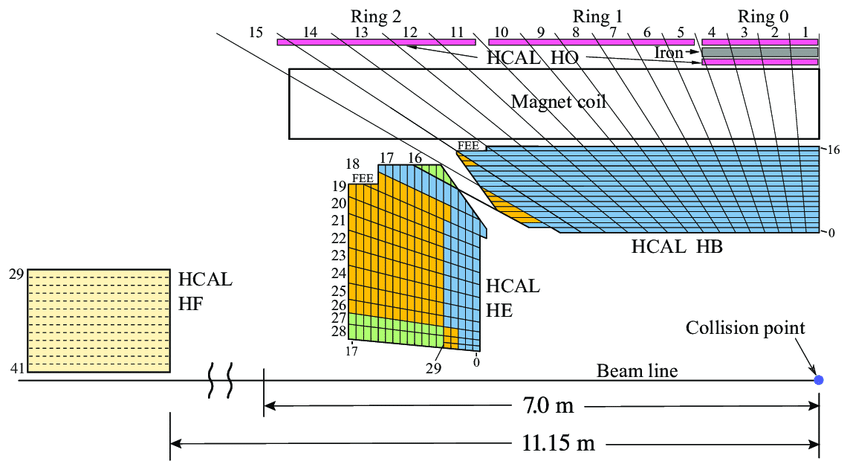
\includegraphics[width=0.6\textwidth]{Images/hcal}
\end{center}
\caption[CMS HCAL structure]{Schematic view of one quarter of the CMS HCAL. Extracted from \cite{intro:exp:hcal}.}
\label{intro:fig:hcal}
\end{figure}

The energy resolution of the HCAL is designed to be approximately
\begin{equation}
\left(\frac{\sigma_E}{E}\right)^2 = \left(\frac{100\%}{\sqrt{E}}\right)^2 + (4.5\%)^2.
\end{equation}

This was confirmed with cosmic and test beam data \cite{intro:exp:hcal_res}, as the hadronic energy resolution of the barrel HCAL and ECAL combination was measured to be
\begin{equation}
\left(\frac{\sigma_E}{E}\right)^2 = \left(\frac{84.7\%}{\sqrt{E}}\right)^2 + (7.4\%)^2.
\end{equation}

\subsubsection{The Muon System}
\label{intro:sec:subdet_muon}

Muons are produced in several physical processes, so the precise measurement of their momenta is key for both Standard Model studies and new physics searches. However, muons interact poorly with the calorimeters and the inactive material, so they are able to travel outside the magnet. To detect them, the CMS Muon System \cite{intro:exp:cms, intro:exp:muon} is located outside the solenoid, inserted between the layers of the iron return yoke of the magnet system. The charge and momentum of the muons can be measured using the magnetic field from the solenoid, providing a complementary measurement to the one performed in the tracker.

The muon chambers are instrumented with three different gas ionization detectors: the \textit{Drift Tube chambers} (DT), the \textit{Resistive Plate Chambers} (RPC) and the \textit{Cathode Strip Chambers} (CSC). Their layout inside the CMS detector is shown in Fig.~\ref{intro:fig:muon}. In the three cases, when a muon transverses the subdetector, the gas inside the chambers is ionized, creating electric signals that are read out by dedicated electronics and are associated with several positions inside the chamber where the muon crossed it, known as \textit{hits}. These are combined in each subsystem and then between subsystems to generate the muon candidates, as described in Section~\ref{intro:subsec:muon}.

\begin{figure}
\begin{center}
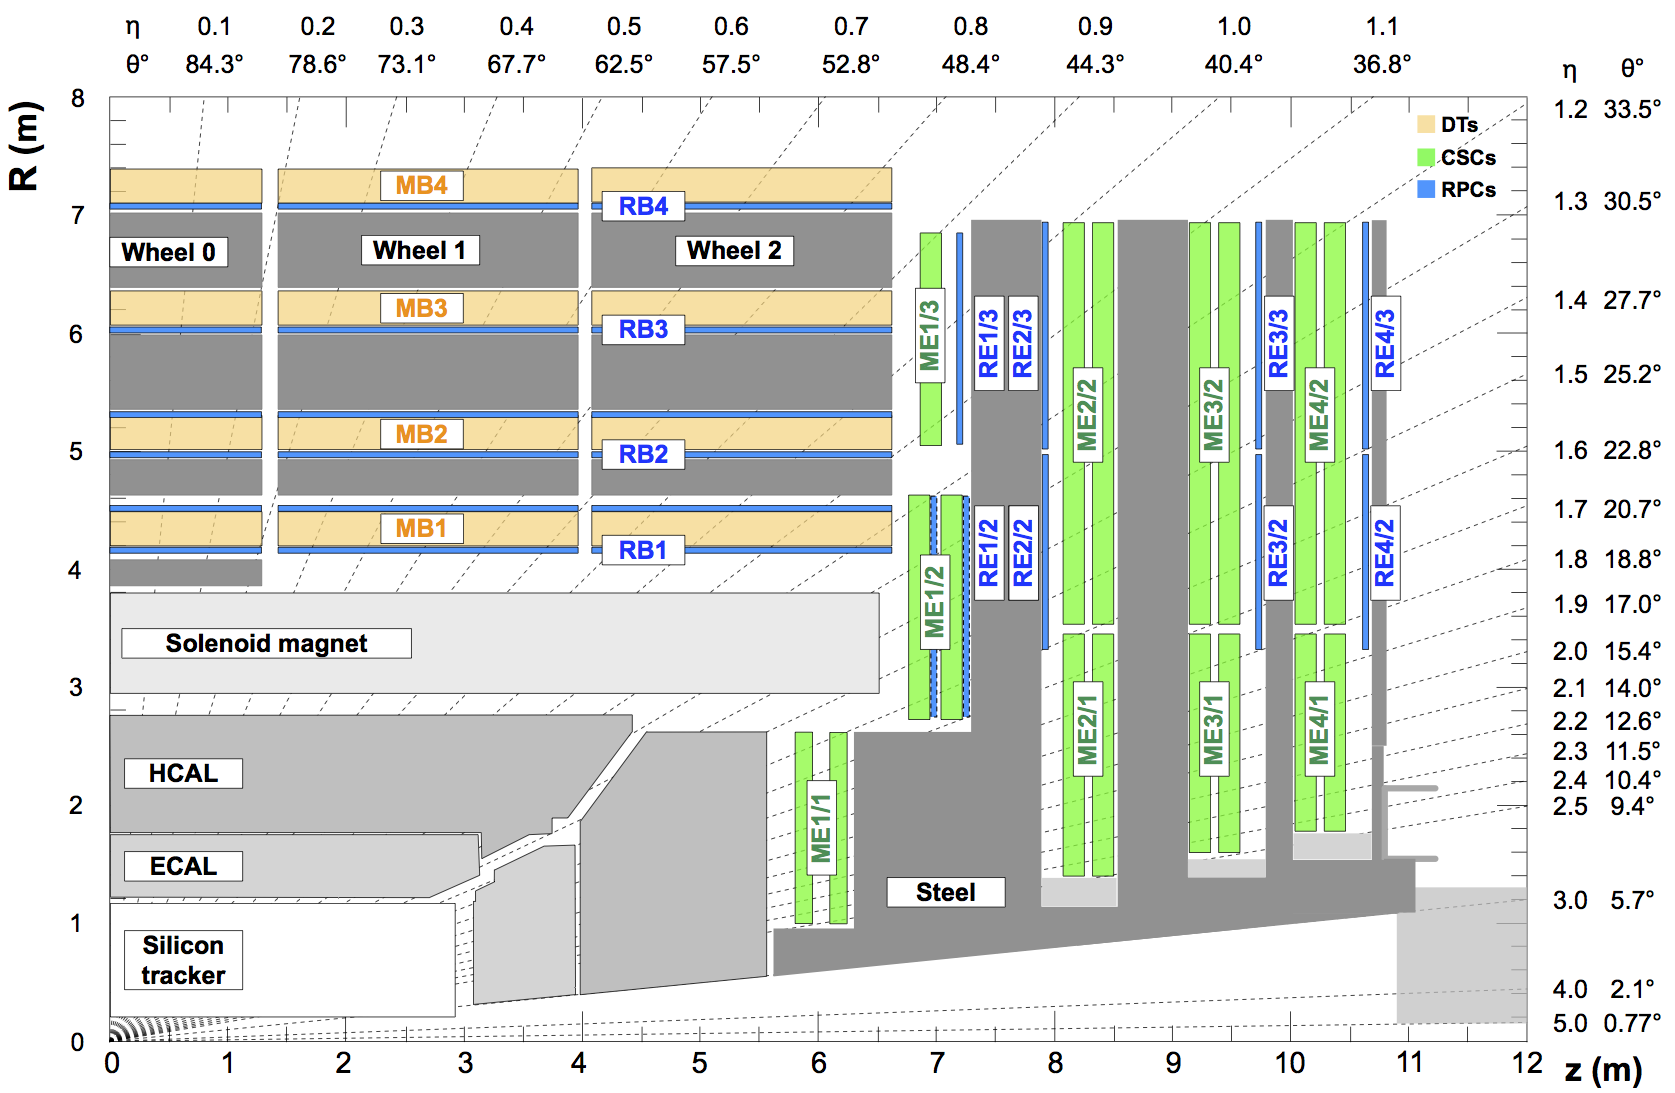
\includegraphics[width=\textwidth]{Images/muonsystem}
\end{center}
\caption[CMS muon detector structure]{Schematic layout of a quadrant of the CMS detector. The location of the muon subsystems is highlighted. Extracted from \cite{intro:id:muon_13tev}.}
\label{intro:fig:muon}
\end{figure}

A brief description of the RPC and CSC systems is shown in the following. The DT system is further described in Section~\ref{intro:sec:dts}.


\paragraph{Cathode Strip Chambers}
CSCs are located in the endcaps, covering $\eta$ regions between $1.2<|\eta|<2.4$. They have shorter drift paths and faster time response, needed in order to cope with the higher muon and other particle rates and the stronger and non-uniform magnetic field found in the endcaps. They are also finely segmented, providing a three-dimensional spatial resolution. CSC detectors have a trapezoidal shape and contain alternate layers of anode wires and cathode stripes, filled with Ar, CO${}_2$ and CF${}_4$ (50\%-40\%-10\%). Similarly to the DT chambers, the detection principle is the ionization of the gas when a muon crosses the chamber, inducing signals used to provide a precise measurement of the position, with an spatial resolution of 40-150~$\mu$m.

\paragraph{Resistive Plate Chambers}
RPCs are installed in both the barrel and endcaps, reaching up to $|\eta|<1.9$. They are formed by two parallel plates, an anode and a cathode, separated by a mixture of gases. The detector works in avalanche mode: when the muon crosses a chamber, an electromagnetic cascade is produced by the high electric field, inducing a signal read out by the strips located in the outer surface. As the segmentation is very poor, so is the spatial resolution (0.8 - 1.2~cm), although they are faster detectors than both DTs and CSCs, with a time resolution better than 3~ns. Therefore, they are particularly useful in detecting the bunch crossing associated to the muon track, even in high PU scenarios.




\subsection{CMS trigger system}

Given the high luminosity provided by the LHC and the large amount of information coming from the detector cells, a huge data rate is produced by the experiment ($\sim$TB/s). However, most of the collisions result in low energy $pp$ collisions, not meant to be studied in the experiment, while the processes of interest for the LHC physics program have smaller cross sections by several orders of magnitude, as shown in Fig.~\ref{intro:exp:xs}. Therefore, a trigger system which reduces the event rate while keeping the events interesting for CMS physics analysis is needed. 

The CMS trigger system \cite{intro:exp:cms_trigger} is implemented in two steps: the Level-1 (L1) Trigger, a hardware-based system, and the High Level Trigger (HLT), which is software-based.

\begin{figure}[h!]
\begin{center}
\includegraphics[width=0.5\textwidth]{Images/crosssections2012_v5}
\end{center}
\caption[Cross sections summary]{Summary of cross section calculations at NLO or NNLO at the LHC and Tevatron. Extracted from \cite{intro:exp:xs}.}
\label{intro:exp:xs}
\end{figure}


\subsubsection{The Level-1 trigger}

The L1 Trigger takes the data coming from the subdetectors and selects events at a rate of up to 100 kHz from the incoming 40 MHz, making decisions within a time interval of less than 4~$\mu$s after the collision. Due to the timing constrains, the L1 cannot run the whole reconstruction of the physics objects and their trajectories. Instead, it produces the so-called L1 \textit{candidates}, low resolution physics objects that rely only on the inputs coming from the calorimeters and the muon system.


Fig.~\ref{intro:exp:l1trigger_sketch} shows an schematic structure of the L1 trigger. The information of the energy deposits in the HCAL and ECAL subdetectors is processed by the \textit{calorimeter trigger}. The transverse energy measured in the calorimeters is transmitted to the calorimeter trigger in form of \textit{trigger primitives}, which are then combined into trigger object candidates: electrons, photons, hadronic $\tau$ ($\tau_h$) leptons, jets and energy sums. As only the information of the calorimeter can be used, both electrons and photons are reconstructed together as L1 $e/\gamma$ objects by clustering energy deposits. The L1 $\tau_h$ objects are identified from their decays into charged or neutral pions. These pions are reconstructed with a clustering algorithm adapted from the L1 $e/\gamma$ algorithm. A key feature of the L1 $\tau_h$ objects is their isolation, which allows to discriminate them from QCD jets, keeping background under control and increasing the purity. L1 jets are reconstructed through energy deposits centred around a local maximum. The total sum of the transverse energy over all the energy deposits can provide an estimation of the missing transverse energy.

 

\begin{figure}[h!]
\begin{center}
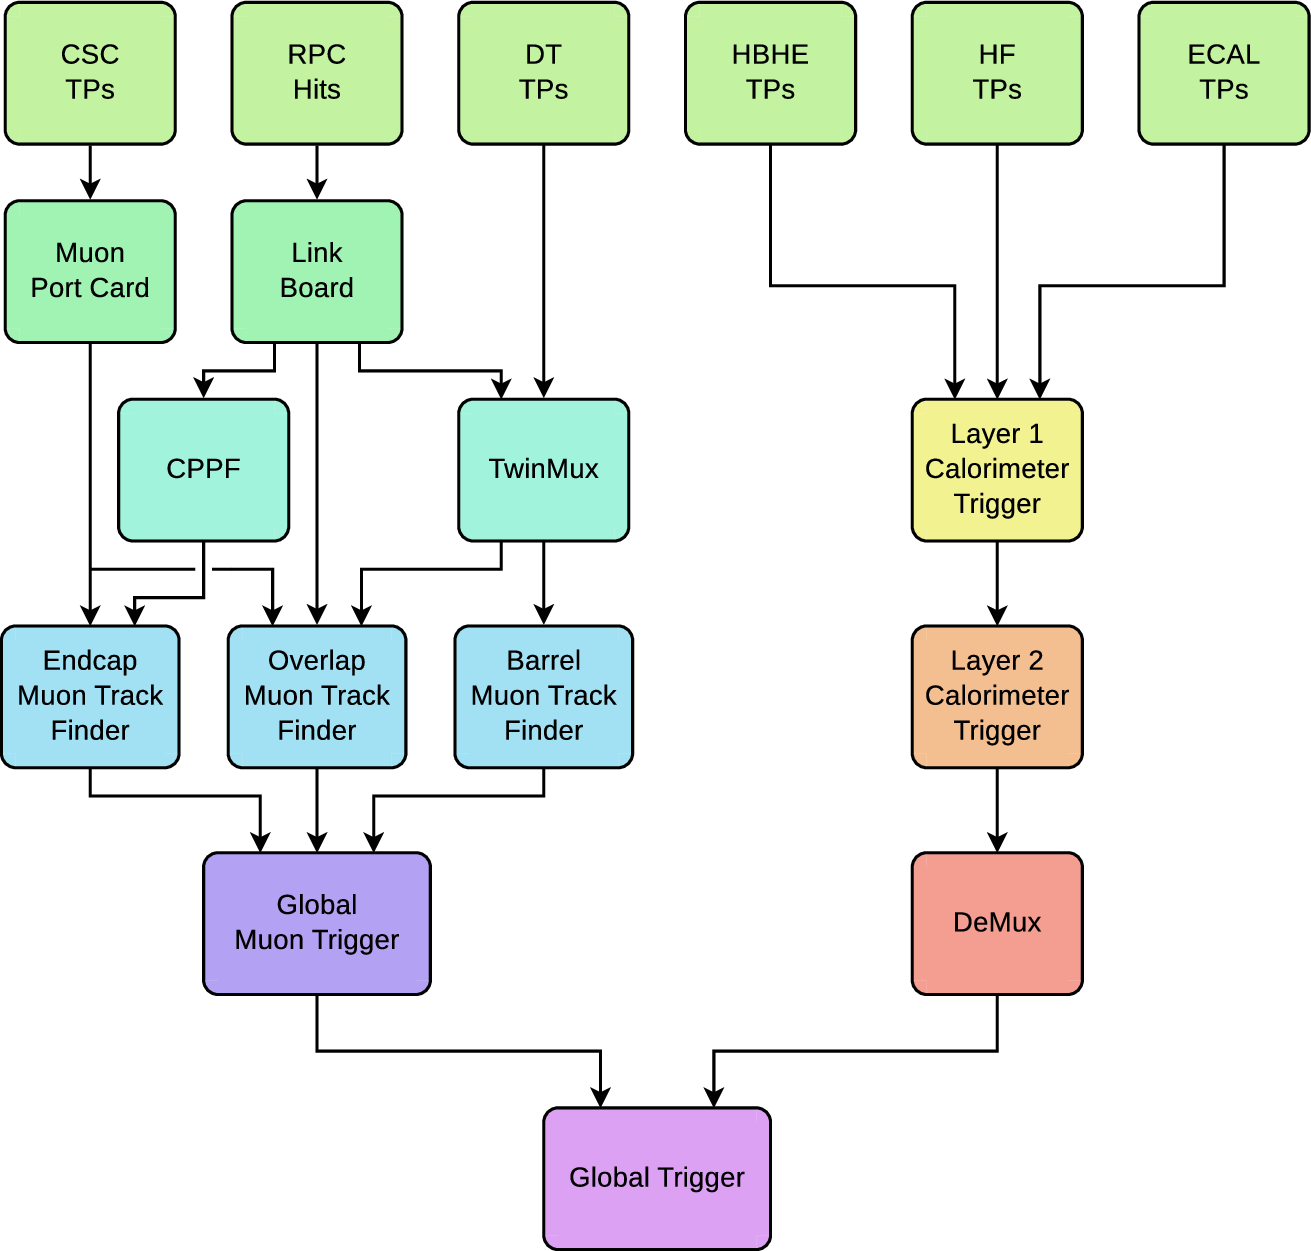
\includegraphics[width=0.6\textwidth]{Images/l1trigger}
\end{center}
\caption[CMS L1 trigger system]{Diagram of the CMS L1 trigger system. Extracted from \cite{intro:l1_13tev}.}
\label{intro:exp:l1trigger_sketch}
\end{figure}

The DT and CSC subdetectors generate, at detector level, their trigger primitives by reconstructing segments on each chamber out of the received hits. These trigger primitives, together with RPC hits, are collected in the \textit{muon trigger}. In the barrel, the Barrel Muon Track Finder (BMTF) uses the information from the DT and RPC subdetectors, whose information is merged into trigger primitives in the \textit{TwinMux} system. The Endcap Muon Track Finder (EMTF) uses the data from the CSC and RPC detectors, while the Overlap Muon Track Finder (OMTF) makes use of the information coming from the three subdetectors. The three track finders create muon candidates with a $p_T$, $\eta$, $\phi$ and a quality criteria that are then sent to the Global Muon Trigger ($\mu$GMT), which orders them by $p_T$ and quality and removes the duplicates.

The candidates coming from the calorimeter and muon trigger are finally sent to the Global Trigger ($\mu$GT), which decides if the event is kept or discarded based on L1 selection algorithms commonly called \textit{seeds}. Basic seeds can be built by applying thresholds on kinematic observables of one or more objects of one type (or \textit{collection}), e.g. requiring one electron with $p_T$ bigger than some value. More complicated seeds can also be included by applying thresholds on objects coming from different collections (often called \textit{cross-triggers}) or on more elaborated observables, as $\Delta\eta$ or $\Delta R$. A full set of seeds is known as the \textit{L1 Menu}.

The L1 menu is configured to perform optimally under different luminosity and pile-up conditions, so the thresholds are constantly updated to keep the rate under 100 kHz. Different luminosity settings (\textit{columns}) are available, each of them including different sets of seeds (or even the same seed with different thresholds), so the menu can be adapted to the LHC running conditions during each fill. Additionally, to reduce the rate coming from a particular seed, this seed could be \textit{prescaled}, so only a predefined fraction of events that satisfy this seed's selection will actually trigger.

When designing a new seed to be included in the L1 menu, it's very important that the rate produced by it fits within the allocated rate budget defined by the different physics groups, trying to achieve an efficiency on the signal as high as possible, so the desired events are kept and move along the rest of the acquisition system.

After one of these selection algorithms is fulfilled, the $\mu$GT sends a L1 trigger signal to all subdetectors. The information collected by them is then packed into an \textit{event}, which is assigned an \textit{event number}. Then, the event continues through the next steps of the online processing before getting stored and analysed.

Even if the L1 trigger is a fully hardware-based system, every stage (from the trigger primitive generation to the Global Trigger) has its own software \textit{emulator}, a C++ code that replicates the firmware implementation with a very high accuracy. These emulators are used to monitor the correct functioning of the trigger during data-taking and to evaluate the trigger algorithms over simulated samples.

\subsubsection{The High Level Trigger}

The High Level Trigger (HLT) is the second step of the CMS trigger. It is carried out by a processor farm able to reduce the 100~kHz coming out from the L1 trigger to 1-2~kHz, a bandwidth compatible with the data acquisition capabilities, with a processing time of hundreds of ms. The full detector data is taken as input, performing a reconstruction very close to offline. Some algorithms are even shared between HLT and offline reconstructions, such as Particle Flow (see Section~\ref{intro:sec:id}); others are a simplified version of the offline algorithm, as is the case of the tracking.

HLT candidates are seeded by L1 objects and reconstructed around them. Their reconstruction is performed in a sequence of steps, mainly reconstruction modules and selection filters, groups into \textit{paths}. The full HLT selection, or HLT \textit{menu}, consists of hundreds of paths. Some of them are used for physics; others, the \textit{monitoring} paths, for efficiency computation or background studies. As in the L1 menu, the HLT can have several columns and its trigger paths can or cannot be prescaled.

\subsection{Data Acquisition and Computing systems}


The CMS Data Acquisition System (DAQ) is the system responsible for performing the read-out of all subdetectors after the event selection performed by the L1 trigger, building the events from the fragments delivered by each subdetector, and processing them in a computer farm called the \textit{Event Filter Farm}, where the HLT selection code is run. A selection is done based on the HLT decision, such that any given event is either discarded or sent to storage \cite{intro:exp:cms}.

The output rate of the HLT system is still in the order of 1~kHz. With the large granularity of the CMS detector, the event size is approximately 1~MB. The combination of both leads to petabytes of data produced per year, something not possible to store nor process in the traditional way (i.e.~in the computing resources of the laboratory).


CMS is characterized by being a detector with a very high rate (order of hundreds of Hz) and producing big amounts of data (given that each event has an average size of 1~MB). The combination of both leads to petabytes of data produced per year, something not storable in the traditional way (i.e.~in the computing resources of the laboratory). Instead, CMS makes use of the World-wide LHC Computing Grid (WLCG) \cite{intro:exp:wlcg_1, intro:exp:wlcg_2}, a network created between more than 100 institutes around the world that helps spreading the work and resources necessary to store and analyse the data.

The CMS offline computing system \cite{intro:exp:cms_computing} is arranged in four tiers, geographically distributed, in order to benefit from the resources and expertise from several ins\-ti\-tu\-tes and achieve redundancy amongst multiple centres. First, a single Tier-0 centre at CERN accepts data from the CMS DAQ system, performing a prompt reconstruction of the raw data and creating \textit{datasets} by grouping events with particular physics objects or conditions. The Tier-0 distributes raw and processed data to the seven Tier-1 centers, located in several CMS collaborating countries, such as the Tier-1 centre at PIC (Barcelona, Spain). These centres perform reconstruction, calibration and other data-intensive tasks. They provide the datasets to numerous Tier-2 centres, smaller but with substantial CPU resources, providing capacity for analysis, calibration activities and the production of simulated Monte Carlo (MC) events. CIEMAT (Madrid, Spain) is one of these Tier-2 centres. Finally, Tier-3 centres provide interactive resources for local groups.

The CMS Collaboration uses various data formats, depending on the level of complexity and information required. The RAW format, coming from the Tier-0, is the one that includes all the event information, requiring the most size per event. Then, Tier-1 and Tier-2 centres produce reconstructed (and re-reconstructed) formats from the RAW information. Finally, the data format that contains all the needed information for performing CMS analysis with all reconstructed objects but an smaller size is the Analysis Object Data (AOD). Similar formats reduced in size are miniAOD and nanoAOD, both used in the analyses presented in this thesis. In all cases, data is stored in ROOT \cite{intro:exp:root} files, which contain all the event object information and kinematics. A ROOT file has a tree-like structure with the variables as branches.

A common software framework, the CMS Software (CMSSW), is used in the collaboration for the different analyses. It is an object-oriented structure based on C++ and python, constantly evolving during the different data-taking periods. It contains all services needed to perform simulation, calibration, alignment and reconstruction and the code run in the HLT. 

\section{The CMS Drift Tube system}
\label{intro:sec:dts}

The CMS Drift Tube (DT) system is the subsystem in charge of muon trigger, reconstruction, and identification in the barrel wheels, covering $|\eta|<1.2$. DT chambers are characterized by having a very good single-point position resolution (80-120~$\mu$m) and an adequate timing resolution. The basic element of these chambers is the drift cell, depicted in Fig.~\ref{intro:fig:dtcell}. These cells have a size of 42$\times$13 cm${}^2$ and a length of approximately 2.4~m and are filled with a gas mixture of argon and carbon dioxide (85\%/15\%). Inside the DT cell there is a central wire at a high voltage of 3600~V, two electrodes (cathodes) on the sides at -1800~V, and two electrodes above and below the wires at +1200~V (strips). When a charged particle (a muon) crosses the cell, it ionizes the gas creating electrons that drift towards the wire with a constant velocity of about 54~$\mu$m/ns. Given the cell sizes, the maximum drift time (from one of the walls to the wire) is almost 400~ns. Once the drift time is known, the position can be obtained by its relation with the drift velocity,
\begin{equation}
x_\text{drift} = v_\text{drift}\cdot t_\text{drift}.
\end{equation}

\begin{figure}
\begin{center}
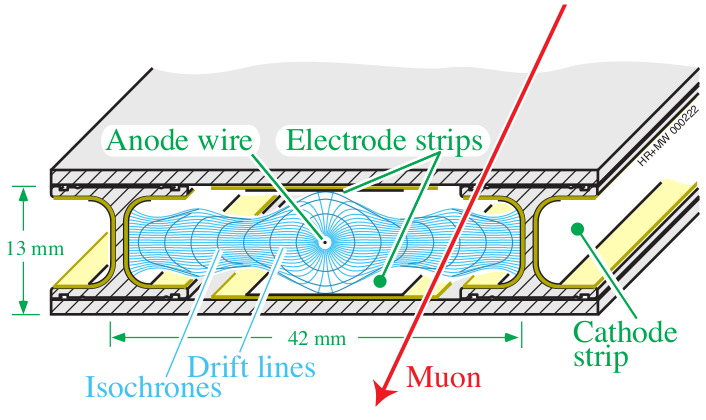
\includegraphics[width=0.5\textwidth]{Images/Celda.png}
\end{center}
\caption[Drift Tube cell]{Sketch of a drift cell showing drift lines and isochrones. Extracted from \cite{intro:exp:cms}.}
\label{intro:fig:dtcell}
\end{figure}

Fig.~\ref{intro:fig:dtwheel} shows an sketch of one of the five wheels of the CMS barrel. Each wheel is divided in 12 \textit{sectors} in azimuthal angle. Each sector consists of four \textit{stations}, labelled from MB1 to MB4 (except sectors 4 and 10, which have two MB4 stations each). Each chamber includes three \textit{superlayers} (SL), described in Fig.~\ref{intro:fig:dtchamber}, from SL1 to SL3. SL1 and SL3 are oriented in the $\phi$ direction, while the second one is orthogonal to them and is oriented in the $z$ direction. In the MB4 stations, only the two $\phi$ SL are available. Each SL includes four \textit{layers} staggered by half a cell. This layout helps to resolve if a muon crossed a DT cell by the left or the right of the wire (also known as \textit{laterality}). All this redundancy helps improving the efficiency and resolution of the system, making it able to cope with situations of dead zones in the detector, such as the space between wheels, electromagnetic showers produced in the chambers by very high $p_T$ muons or the inefficiencies appearing in the DT cells after radiation damage (see Section~\ref{dts:sec:performance}).

\begin{figure}
\begin{center}
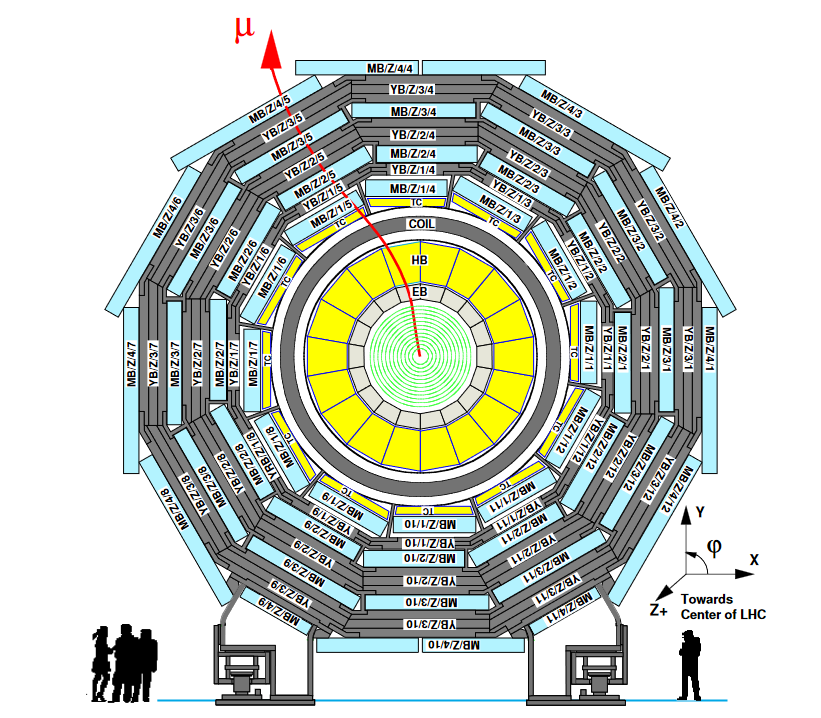
\includegraphics[width=0.5\textwidth]{Images/dtwheel.png}
\end{center}
\caption[CMS barrel muon Drift Tube chambers layout]{Layout of the CMS barrel muon DT chambers in one of the five wheels. Extracted from \cite{intro:exp:cms}.}
\label{intro:fig:dtwheel}
\end{figure}

\begin{figure}
\begin{center}
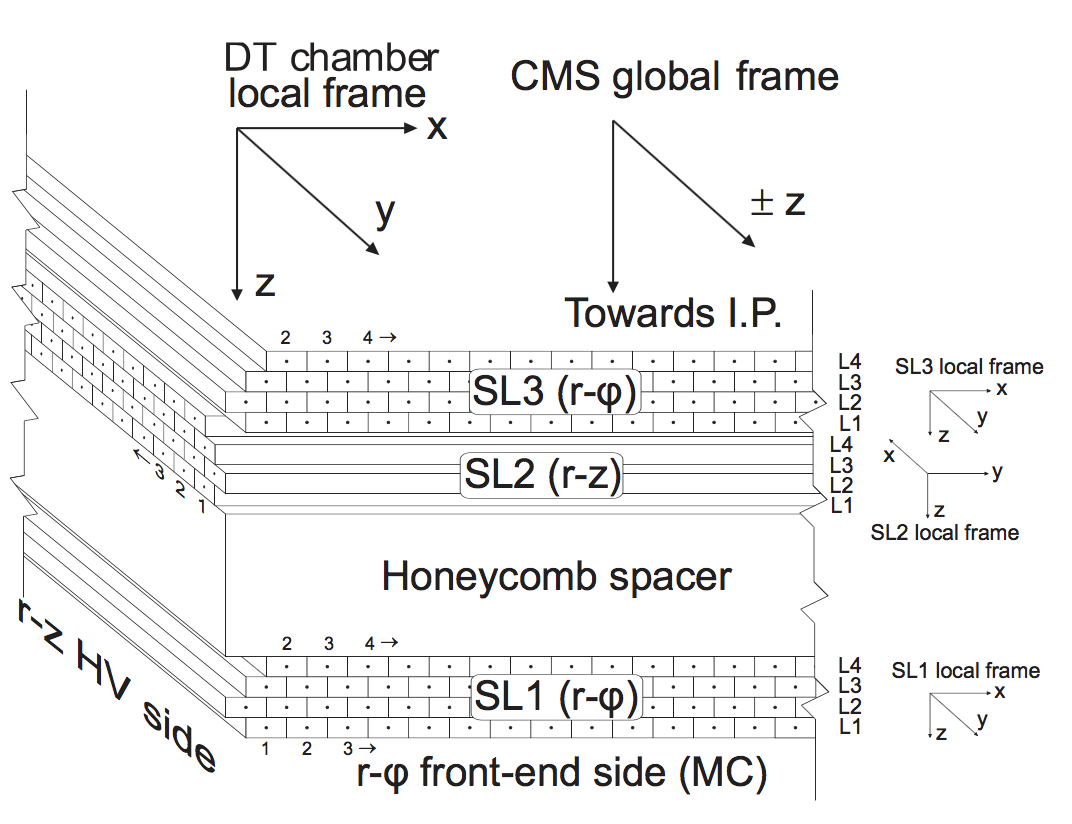
\includegraphics[width=0.5\textwidth]{Images/DT_Chamber.png}
\end{center}
\caption[DT Chamber structure]{Schematic view of a DT chamber. Extracted from \cite{intro:exp:dt_calib}.}
\label{intro:fig:dtchamber}
\end{figure}

\subsection{The DT trigger system}

The DT trigger system is a structured, robust, and redundant system devoted to the fast detection and reconstruction of the muons crossing the DT chambers. It is able to measure the position and trajectory or the crossing particles and identify the bunch crossing from which they were originated. It is implemented using dedicated electronics located both on-detector (in the so-called \textit{minicrates}) and in the service cavern.

Inside the minicrates, the DT trigger chain starts at the superlayer level in the \textit{Bunch and Track Identifier} (BTI), which combines the signals from the wires and generates a trigger at a fixed time after the passage of the muon.  The association of hits is based on a meantimer technique \cite{intro:exp:meantimer}, which uses the fact that there is a relation between the drift times of any three adjacent layers. From the associated hits, the BTI can obtain the BX, position (with a resolution of 1.4~mm), and direction (with a resolution better than 60~mrad) of the track segments \cite{intro:exp:cms}. After the BTI, the \textit{Track Correlator} (TRACO) attempts to correlate the track segments measured in each r-$\phi$ superlayer, enhancing the parameter resolutions. Finally, the \textit{Trigger Server} (TS) board is composed by two subsystems, one devoted to process the output of the TRACO for the r-$\phi$ segments, and another to process the segments coming from the BTI for the r-z superlayer. In both cases, the TS selects the segments with the highest quality (i.e. higher number of hits used) and transverse momentum. The TS obtains a position resolution of 0.8~mm and a direction resolution of 4~mrad, with an efficiency over 90\% \cite{intro:exp:dt_performance}.

The output from the TS is transmitted via copper-to-optical-fiber translators (CuOF) to the service cavern, where the \textit{TwinMux} systems, running in Xilinx Virtex 7 \textit{Field Programmable Gate Arrays} (FPGA) combines the information from the DT and RPC systems, generating the final trigger primitives that will be sent to the Barrel Muon Track Finder.



\section{The Phase-2 upgrade of the CMS experiment}

During HL-LHC, the accelerator will potentially deliver up to $7.5\times10^{34}$~cm${}^{-2}$s${}^{-1}$ and up to 4000~fb${}^{-1}$ (see Section~\ref{intro:sec:hllhc}). In this scenario, the interaction rate, occupancy, PU levels, and radiation ageing will increase beyond the capabilities of the existing detector and trigger technologies. In the CMS \textit{Phase-2} upgrade program \cite{intro:exp:phase2_upgrade}, the goal is to maintain the excellent performance of the present \textit{Phase-1} detector or even improve it wherever possible under these new challenging conditions throughout the whole operation of HL-LHC.

Two major concerns need to be addressed in the required detector upgrade. The first one is the radiation damage, that would reduce the performance of some subdetectors. The second, the higher PU and particle rate require a better precision on the detector to be able to discriminate particles coming from the interactions. A higher granularity is then needed, specifically in the endcaps. 

Some details on the major detector, trigger, and DAQ elements needing upgrading are given in the following

\paragraph{Tracker}

The silicon tracker will suffer from significant radiation damage by LS3, so it will be completely replaced. To maintain the track reconstruction performance with the higher PU levels, the granularity of the pixel detector and the outer tracker will be increased by almost a factor 4. The new outer tracker will be lighter, providing a better resolution and new pixel disks will be added in the forward regions to extend the acceptance close to $|\eta| = 4$.

\paragraph{MIP Timing Detector}

The MIP Timing Detector (MTD) is a new detector planned for CMS during HL-LHC \cite{intro:exp:mtd}. This detector will allow CMS to measure precisely the production time of minimum ionizing particles (MIP), which could help to assign charged tracks to the correct interaction vertices in the new PU 200 scenario. The detector will be placed as a thin layer between the Tracker and the calorimeters, divided into the barrel ($|\eta|<1.5$) and two endcap sections covering up to $|\eta|=3$. In the barrel, the technology used will be crystal scintillators read out by Silicon Photomultipliers (SiPM), while in the endcap, Low-Gain Avalanche Detectors (LGAD) will be used.

\paragraph{Calorimeter endcaps}

The electromagnetic and hadronic endcap calorimeters will also suffer significant radiation damage by LS3, so they must be replaced. The new replacement is called the \textit{High-Granularity Calorimeter} (HGCAL) \cite{intro:exp:hgcal}, a calorimeter with electromagnetic and hadronic sections and excellent longitudinal and transverse segmentation, providing three dimensional images of showers and a timing measurement.

\paragraph{Muon detectors}

The current barrel muon detectors will be kept for HL-LHC. Their electronics, however, will be upgraded in order to cope with the increased rate and luminosity. A more detailed description of the DT upgrade is shown in Section~\ref{intro:subsec:dt_upgrade}. In the endcap, the current muon system consists of four stations of CSCs and four stations of RPCs. To maintain the trigger acceptance in this region during Phase-2, additional chambers that make use of new detector technologies with high rate capability are going to be added \cite{muontdr}, as shown in Fig.~\ref{intro:fig:muon_phase2}. Two new improved RPC (iRPC) stations will be installed along CSC stations 3 and 4, extending the RPC pseudorapidity coverage to $|\eta|<2.4$. In the $1.6<|\eta|<2.8$, new \textit{Gas Electron Multiplier} (GEM) chambers will be installed. These new chambers provide a precise measurement of the muon bending angle and help controlling the trigger rate while increasing the trigger efficiency and the operational resilience of the system. Three new GEM superchambers (that group two or six GEM chambers) will be installed, named as GE1/1, GE2/1 and ME0.

\begin{figure}[h!]
\begin{center}
\includegraphics[width=\textwidth]{Images/muonsystem_phase2}
\end{center}
\caption[CMS structure after the Phase-2 upgrade]{Longitudinal view of a quadrant of the CMS detector after the installation of the HGCal and the new muon chambers. Extracted from \cite{l1tdr}.}
\label{intro:fig:muon_phase2}
\end{figure}


\paragraph{Trigger}

The latency of the present L1 trigger is limited to 3.4~$\mu$s by the tracker readout. During Phase-2, for the first time the tracker information will also be used at trigger level. The tracker trigger will perform pattern recognition to reconstruct the tracks of primary particles with $p_T > 2$~GeV, discarding as many low energy tracks as possible. The reconstructed tracks will then be matched with the muon and calorimeter information, increasing latency to 12.5~$\mu$s. This will require upgrades of the readout electronics in some of the existing sub-detectors: barrel calorimeter, DTs (further described below) and CSCs. New detector electronics must be designed to sustain larger L1 rate, of 500(750) kHz for PU 140(200) scenario, keeping typical values of $p_t$ and energy thresholds as in a Phase-1 trigger menu.

\paragraph{Data Acquisition and Trigger Control}

The DAQ system will be upgraded to implement the increasing of bandwidth and computing power needed to accommodate the larger event size and L1-trigger rate. Compared to Phase-1, bandwidth and computing power will increase by factors of about 10(15) and 15(30) for operation at PU 140(200).

~\\Apart from these changes, some upgrades on the barrel calorimeters electronics, protections against beam background, the luminosity measurement system and software and computing for online and offline analysis are also planned. 


\subsection{Upgrade on the DT Trigger system for Phase-2}
\label{intro:subsec:dt_upgrade}

The DT chambers located in the barrel region of CMS are responsible of muon detection and precise momentum measurement over a wide range of energies. They provide identification, reconstruction and trigger
on muons. During the Phase-2 upgrade \cite{muontdr, l1tdr}, the goal is to maintain or improve the present system performance for trigger and offline reconstruction at the HL-LHC background rates and trigger conditions (500-750~kHz L1 trigger rate and 12.5~$\mu$s latency).

Present DT detectors will remain for HL-LHC operation. Even if the most exposed chambers will suffer from detector ageing at the end of HL-LHC due to radiation damage \cite{muontdr}, the loss of performance is expected to be minor after this period (see Section~\ref{dts:sec:performance}). However, the DT on-detector electronics must be replaced since they are not prepared for the HL-LHC radiation conditions and can't cope with the expected increase of L1 rate foreseen during Phase-2 operation.

In the upgraded DT architecture, only the time digitization of the chamber signals will stay on-detector. This will be performed by the new \textit{On-Board electronics for DT} boards (OBDT). These boards receive signals from each anode wire and assigns them a digital timestamp. The trigger primitive generation, presently performed also on-detector, will be moved from the experimental cavern to the service cavern. In the service cavern, new boards will be installed featuring the latest commercial FPGAs. A new trigger algorithm will be running in these boards, profiting from the full chamber information with the best DT time resolution (few ns), so it can generate DT trigger primitives with a more precise and robust bunch crossing identification, better spatial resolution (close to offline level), and better fakes rejection. This new algorithm is described in Chapter~\ref{dts:chapter:intro}.

Once the DT trigger primitives have been generated, they are sent to the BMTF, where standalone muons are built. Standalone muons and L1 tracks (from the tracker) are sent to the Global Muon Trigger. The output from the Global Muon Trigger is combined with the information from the other trigger subsystems in the Global Trigger. Finally, the Global Trigger calculates a trigger decision based on the L1 menu.



%\bibliographystyle{plain}
%\bibliography{../biblio.bib}

\end{document}

